%ltex: language=de-DE
\chapter{Vorbereitung}
	Um der zweigeteilten Natur des Praktikumsversuchs Sorge zu tragen wird die Diskussion der Vorbereitung in separaten Unterkapiteln
	erfolgen.
	\section{Kalorimetrischer Aufschluss und Brennwertbestimmung}\label{sec:vorbereitung kalorimetrischer aufschluss}
		Versuch 11 beschäftigt sich mit der Theorie sowie der praktischen Durchführung eines kalorimetrischen Aufschlusses
		eines Paraffinöls, welches mit Chlorkohlenwasserstoff verunreinigt ist.\par
		Die durch vollständige Verbrennung frei gesetzte thermische Energie verteilt sich auf die direkt nutzbare und die durch
		etwa Verdampfung abtransportierte und für gewöhnlich verlorene Wärmemenge. Unter Einbezug auch der in der Dampfphase liegenden
		thermischen Energie wird in diesem Zusammenhang vom \textit{Brennwert} eines Stoffes gesprochen.
		Im vorliegenden Versuch soll unter Zuhilfenahme des Kalorimeters C 6000 der Firma \textsc{IKA} der Brennwert einer Paraffinprobe
		bestimmt werden.
		\begin{figure}[h]
			\centering
			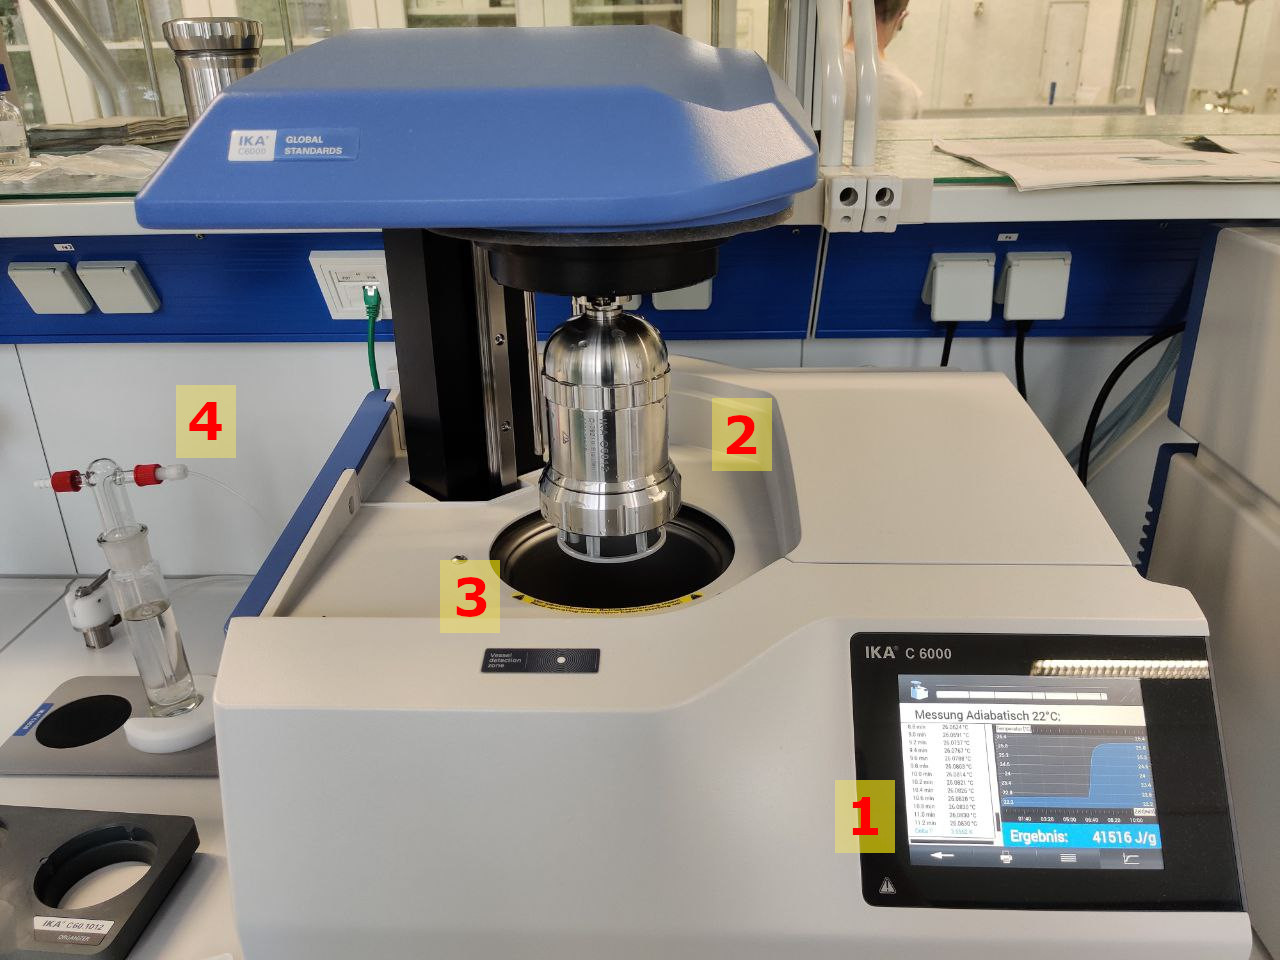
\includegraphics[width=.7\textwidth]{assets/photos/kaloriemeter_aufbau_edit.jpg}
			\caption[Im Versuch verwendetes Kalorimeter]{Im Versuch verwendetes Kalorimeter C 6000 der Firma \textsc{IKA}. Zu sehen 1: Bedienfeld, 2: Druckbehälter, 3: Innenkessel, 4: Entlüftungsstation.}
			\label{fig:kalorimeter aufbau}
		\end{figure}
		Das Funktionsprinzip besteht hierbei aus einer sehr genauen Messung der Temperaturerhöhung eines die Verbrennungskammer umfließenden
		Wassers. Da es hierbei unweigerlich auch Wärmemengenverluste an den Gefäßwänden, Leitungen und dergleichen kommt, muss,
		um entsprechende Kompensationen durchführen zu können, im Vorfeld jeder Messung eine Kalibrierung durchgeführt werden.
		Die Kalibrierung bestimmt hier die Wärmekapazität der Messeinrichtung selbst und folgt der kalorischen Grundgleichung aus \cref{eq:kalorische grundgleichung} \cite{Einstieg.in.die.Physikalische.Chemie.fuer.Nebenfaechler.Bechmann.2016}.
		\begin{equation}
			Q = \Delta T \cdot k = \Delta T \cdot \sum_i \varsigma_i \cdot m_i
			\label{eq:kalorische grundgleichung mit kaloriemeterkram}
		\end{equation}

		\(k = \sum_i \varsigma_i \cdot m_i\) in \cref{eq:kalorische grundgleichung mit kaloriemeterkram} bezeichnet hier einen systemspezifischen Proportionalitätsfaktor, der die kumulierte
		Fähigkeit der einzelnen Systemkomponenenten Wärme aufzunehmen widerspiegelt und muss durch Kalibrierung ermittelt werden. Wie in \cref{sec:theo hintergrund} beschrieben sind hier \(Q\)
		die zugeführte Wärmemenge und \(\Delta T\) die zu messende Temperaturänderung.
		
		Sowohl die eigentliche Messung als auch die Kalibrierung finden unter Zufuhr reinen Sauerstoffs bei \(\approx \SI{30}{\bar}\) statt. Hierbei wird, wie eingangs bereits erwähnt, das Präparat
		vollständig verbrannt während die Temperaturänderung des umliegenden Wassers konstant gemessen wird.\par\medskip
		
		Die zu bestimmende Probe ist ein chloriertes Paraffin (vgl. \crefrange{subfig:paraffin rein}{subfig:paraffin ckw}). So wird beim Versuch über die Bestimmung des Brennwertes des
		Präparates hinaus auch der Massenanteil des Chlors innerhalb der Chlorkohlenwasserstoff-Kette bestimmt. Dies geschieht in einer nachgelagerten konduktometrischen Fällungstitration, die in \cref{sec:titration}
		näher erläutert werden soll.\par\medskip
		Um den beim Aufschluss zu erwartenden Chlorwasserstoff aufzufangen wird in Vorbereitung \SI{50}{mL} 0,2 molarer Natronlauge hergestellt.
		\begin{equation}
			c(NaOH) \cdot V = c_{soll}(NaOH) \cdot V_{soll} \quad \Leftrightarrow \quad V = \frac{c_{soll}(NaOH) \cdot V_{soll}}{c(NaOH)}
			\label{eq:verduennung}
		\end{equation}\\
		Im Versuch steht 1 molare Natronlauge zur Verfügung aus der die gewünschte Konzentration \(c_{soll}(NaOH)\) durch Verdünnung hergestellt werden muss.
		\Cref{eq:verduennung} folgend errechnet sich die zu entnehmende Menge zu
		\begin{align}
			\frac{\SI{0,2}{\mole\per\litre} \cdot \SI{0,05}{\litre}}{\SI{1}{\mole\per\litre}} = \SI{0,01}{\litre}
		\end{align}
		Mit einer Vollpipette vorsichtig entnommen und in einen Messkolben überführt wird die Differenz zum Sollvolumen mit VE-Wasser aufgefüllt.\par\medskip
		%
	\section{Konduktometrische Titration}\label{sec:titration}
		Im vorliegenden Versuch wird nach der Methode der konduktometrischen Titration der Chloridgehalt der Absorberlösung aus Versuch 11 mittels Neutralisation mit
		einer Silbernitratlösung bestimmt. Da hierzu die Ionenkonzentration des Titers möglichst genau bekannt sein muss, wird vorbereitend eine Lösung bekannten Chloridgehalts
		titriert. \nocite{Analytische.Chemie.I.Ritgen.2019}
		\begin{figure}[h]
			\centering
			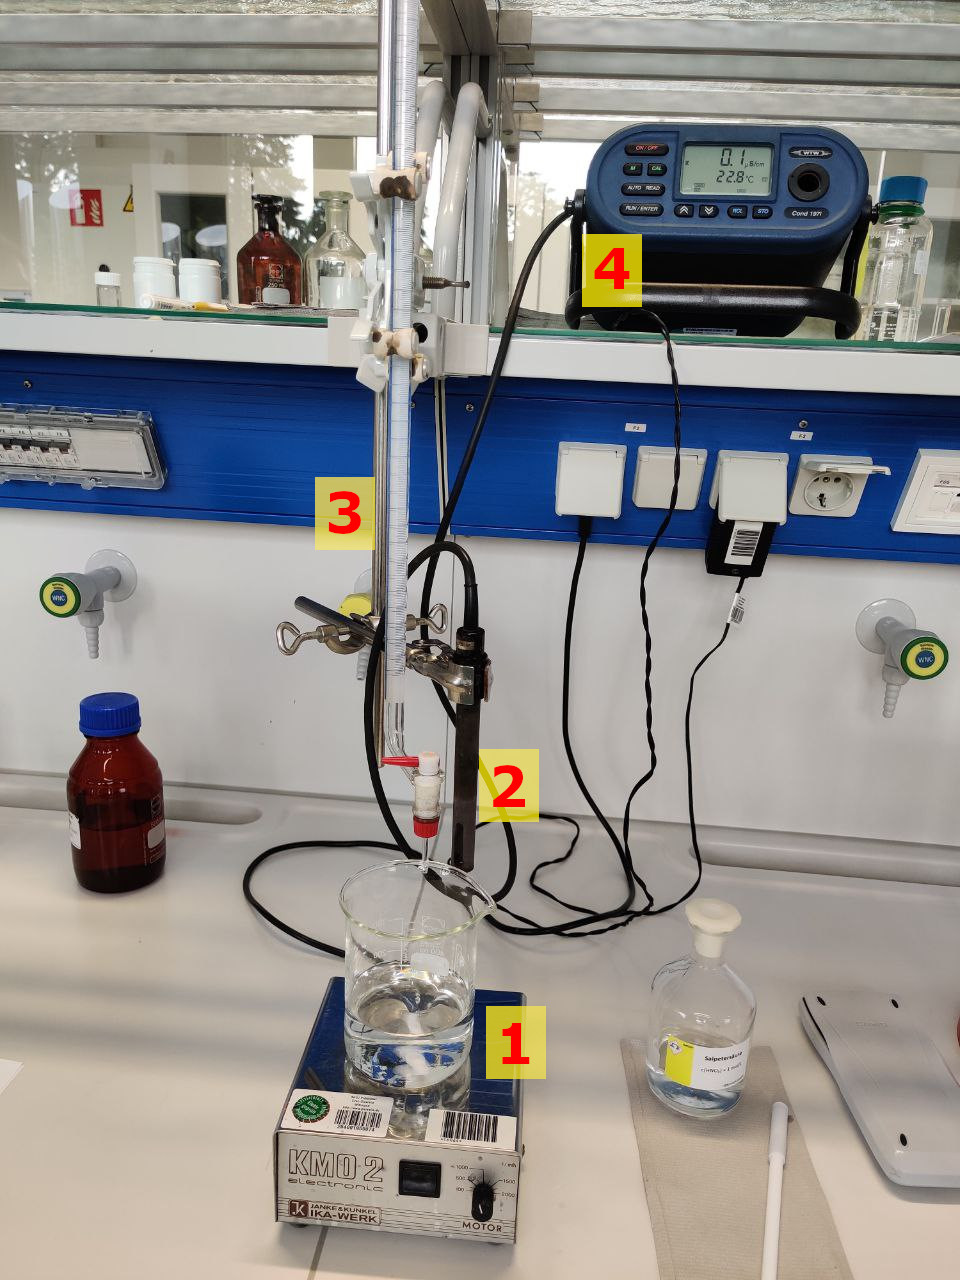
\includegraphics[width=.7\textwidth]{assets/photos/aufbau1_edit.jpg}
			\caption[aufbau Titration]{Aufbau der konduktometrischen Titration. 1: Magnetrührer mit Becherglas und Titrand, 2: Elektroden zur Leitwertmessung, 3: Bürette, 4: Leitwertmessgerät.}
			\label{fig:aufbau titration}
		\end{figure}
		%
		\subsection{Lösung bekannten Chloridgehaltes}\label{sec:bekannter chloridgehalt}
			Zur Herstellung einer Lösung bekannten Chloridgehalts wird Natriumchlorid (Kochsalz) auf der Laborwaage möglichst genau eingewogen
			und in einem Messkolben durch Auffüllen mit VE-Wasser gelöst. Ziel ist eine Chloridkonzentration von \(c(Cl^{-}) \approx \SI{0,1}{\mole\per\litre}\).
			\begin{equation}
				m = \left[M(Cl^{-}) + M(Na^{+})\right] \cdot c(Cl^{-}) \cdot V
				\label{eq:masse NaCl}
			\end{equation}

			Mit den molaren Massen von \(M(Cl^{-}) \approx \SI{35,450}{\gram\per\mole}\) und \(M(Na^{+}) \approx \SI{22,98977}{\gram\per\mole}\) sowie
			dem herzustellenden Volumen von \(V = \SI{50}{\milli\litre}\) ergibt sich mit \cref{eq:masse NaCl} eine einzuwiegende Masse des Salzes
			von gemäß \SI{292,2}{mg}. Mit einer tatsächlich eingewogenen Masse von\\
			\(\SI{(298,8 \pm 0,1)}{\milli\gram}\) führt dies wiederum in guter Näherung zu einer Konzentration von
			\begin{align}
				c(Cl^-) &= \frac{m}{\left[M(Cl^-) + M(Na^+)\right] \cdot V}\nonumber \\
						&= \frac{\SI{292,2}{\milli\gram}}{\left[\SI{35,450}{\gram\per\mole} + \SI{22,98977}{\gram\per\mole}\right] \cdot \SI{0,05}{\litre}}\nonumber\\
						&\approx \SI{0,1}{\mole\per\litre}
				\label{eq:konzentration Cl}
			\end{align}

			Von der hergestellten Lösung werden \SI{25}{\milli\litre} entnommen und innerhalb eines Becherglases mit \SI{200}{\milli\litre}
			VE-Wasser verdünnt.
		\subsection{Titerbestimmung}\label{sec:titerbestimmung}
			Das Becherglas aus \cref{sec:bekannter chloridgehalt} wird mit einem Rührstäbchen versehen auf einen Magnetrührer gestellt und
			das in einem Stab kombinierte Elektrodenpaar des Konduktometers in einem über dem Becherglas befindlichen Stativ so arretiert, dass
			die Kontaktflächen der Elektroden möglichst tief in die Lösung eintauchen\footnote{Hierbei ist darauf zu achten, dass der Elektrodenstab möglichst frei von Kontamination ist.}.

			Nach Einschalten des Magnetrührers wird in \SI{2}{\milli\litre}-Schritten Silbernitratlösung zu titriert und bei jedem Titrationsschritt die
			momentane Leitfähigkeit der Lösung am Konduktometer abgelesen und aufgezeichnet. Nahe des Äquivalenzpunktes werden die Titrationsschritte auf
			etwa \SI{0,5}{\milli\litre} reduziert um das Minimum der Leitfähigkeit möglichst genau zu lokalisieren. Ist der Äquivalenzpunkt erreicht wird die Schrittweite
			der Titration wieder erhöht und so lange Silbernitratlösung zugegeben, bis etwa \SI{20}{\milli\litre} über den Äquivalenzpunkt hinaus verbraucht sind.